\chapter{曲面}


\section{曲面}

\begin{definition}[曲面][def:9.1]
\index{q@曲面}
    设 $X$ 是一个拓扑空间，如果
    \begin{enumerate}[(i)]
        \item $X$ 是 Hausdorff 空间.
        \item $X$ 是第二可数的.
        \item 对任意 $x \in X$，存在 $x$ 的一个邻域同胚于 $\mathbb{E}^2$ 或 $\mathbb{E}^2_+$，该同胚将 $x$ 映为 $0 \in \mathbb{E}^2$ 或 $0 \in \mathbb{E}^2_+$.
    \end{enumerate}
    则称 $X$ 为一个\colorbf{曲面}.
\end{definition}
\vspace{-1 em}
\begin{figure}[h]
    \centering
    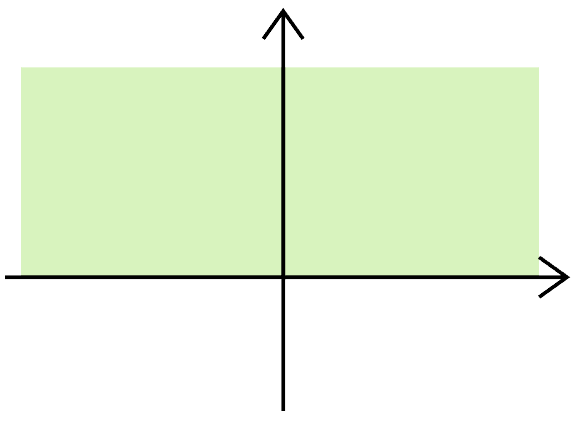
\includegraphics[width=0.25\textwidth]{fig/9.1.png}
    \captionof{figure}{上半平面$\mb{E}^2_+$}
\end{figure}



\begin{instance}
    \begin{center}
        \vspace{-2 em}
        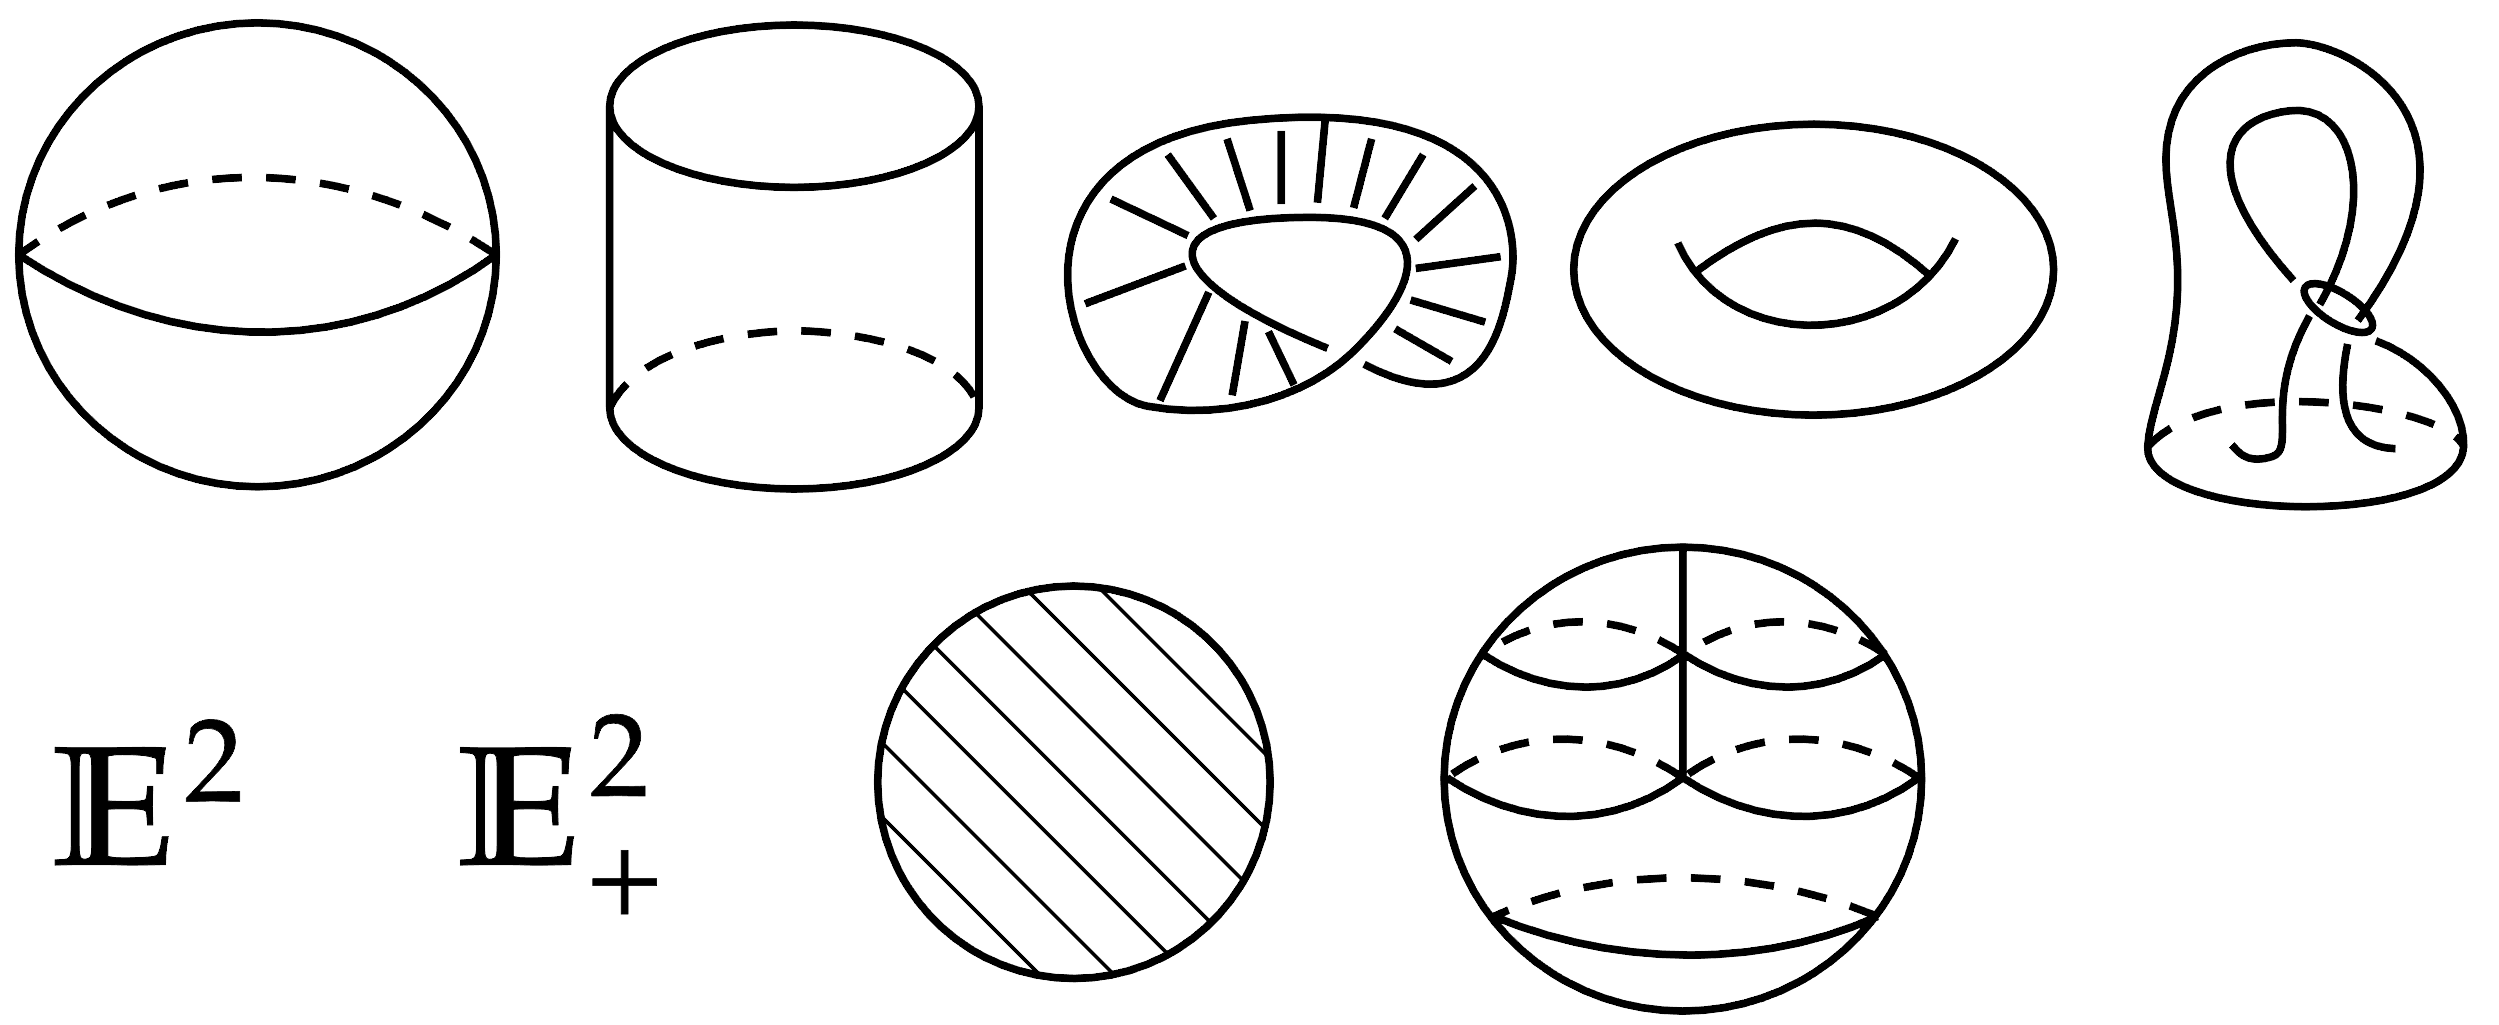
\includegraphics[width=0.8\textwidth]{fig/9.2.png}
        \captionof{figure}{曲面的例子}
    \end{center}
\end{instance}

\begin{instance}
    三角形的商空间不是曲面，其原因在于在任意边上取一点，它的邻域由三个半径相等的半圆构成，与$\mb{E}^2$和$\mb{E}^2_+$均不同胚.\par
    锥面 $\{(x,y,z) \in \mathbb{E}^3 \mid x^2+y^2=z^2\}$ 不是曲面.因为两个圆锥的交点处没有与$\mb{E}^2$或$\mb{E}^2_+$同胚的曲面.\par
    \vspace{-1 em}
    \begin{minipage}[t]{0.49\textwidth}
        \begin{center}
        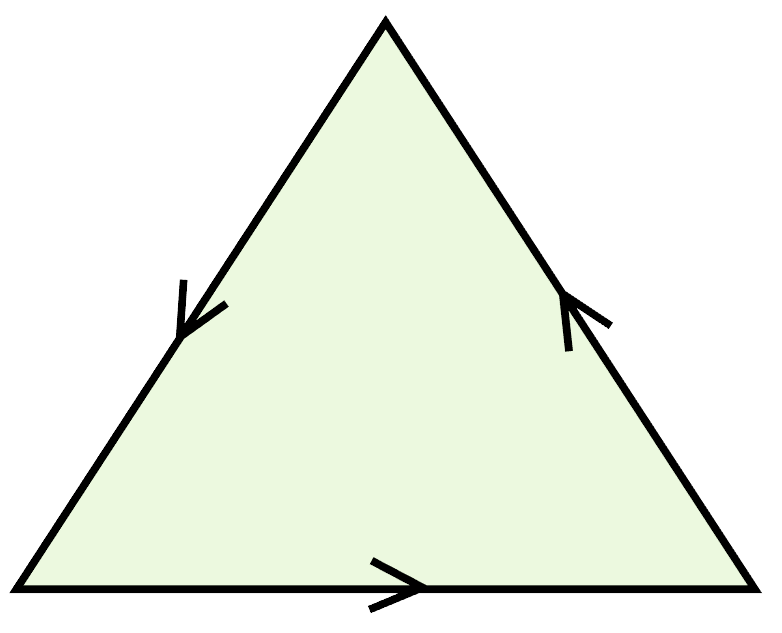
\includegraphics[width=0.5\textwidth]{fig/9.3.png}
        \captionof{figure}{}
        \end{center}
    \end{minipage}
    \begin{minipage}[t]{0.49\textwidth}
    \begin{center}
        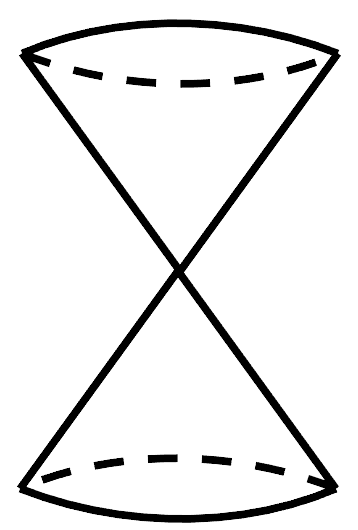
\includegraphics[width=0.3\textwidth]{fig/9.4.png}
        \captionof{figure}{}
    \end{center}
    \end{minipage}    
\end{instance}


\begin{definition}[边界][def:9.2]
    设 $S$ 是一个曲面，若 $x \in S$ 有一个邻域同胚于 $\mathbb{E}^2_+$ 且该同胚将 $x$ 映为 $0 \in \mathbb{E}^2_+$，则称 $x$ 为 $S$ 的一个\colorbf{边界点}.
    $S$ 的边界点的集合称为 $S$ 的\colorbf{边界}，记为 $\partial S$.\par
    若紧致曲面 $S$ 满足 $\partial S = \varnothing$，则称其为\colorbf{闭曲面}.
\end{definition}
依照上述定义，球面、环面、克莱因瓶和射影平面均为闭曲面.

\begin{definition}[曲面定向][def:9.3]
    若曲面 $S$ 包含一个嵌入的莫比乌斯带，则称 $S$ 是\colorbf{不可定向的}.否则称其为\colorbf{可定向的}.
\end{definition}
\begin{figure}[h]
    \centering
    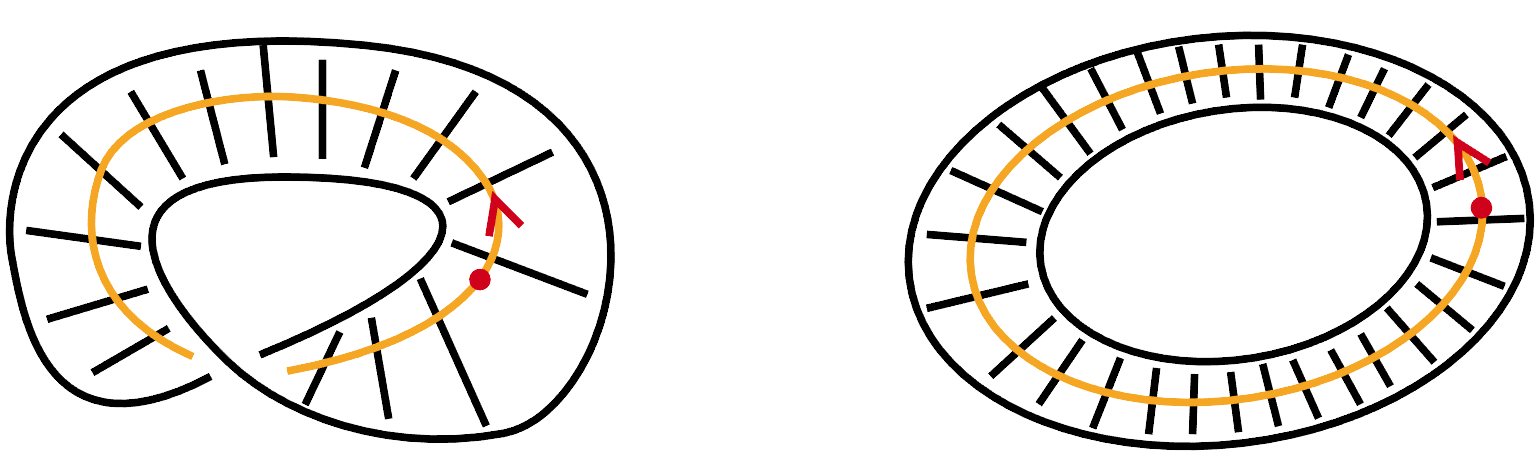
\includegraphics[width=0.75\textwidth]{fig/9.5.png}
    \captionof{figure}{不可定向曲面与可定向曲面}
\end{figure}

\begin{instance}
    $\mathbb{R}\mb{P}^2$ 和克莱因瓶是不可定向的.
\end{instance}

\begin{theorem}[][thm:9.1]
    设 $S_1, S_2$ 是曲面，且 $S_1 \cong S_2$.则 $S_1$ 可定向 $\iff S_2$ 可定向.
\end{theorem}
这表示一个曲面是否定向是一个拓扑性质.

\begin{definition}[连通和][def:9.4]
\index{l@连通和}
\end{definition}
\begin{instance}
    球面$\#$环面 $\cong$ 环面.\par
    \begin{center}
        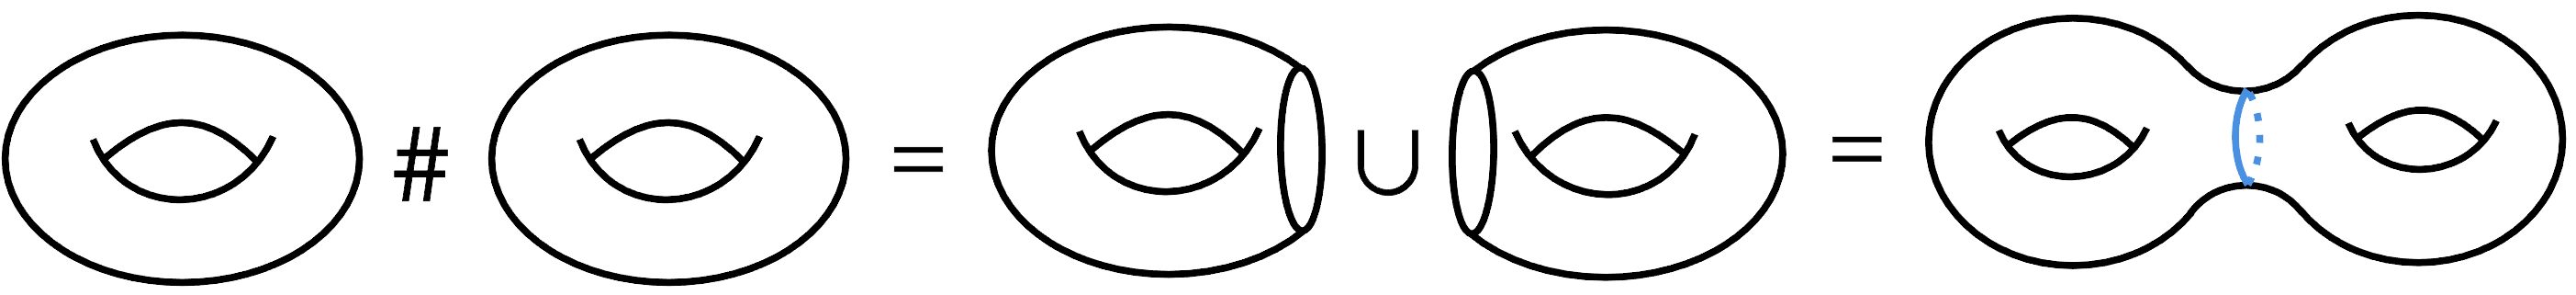
\includegraphics[width=0.98\textwidth]{fig/9.6.png}
    \captionof{figure}{$T^2\# T^2$}
    \end{center}
\end{instance}


\begin{remark}
    连通和运算与我们移除的具体开圆盘以及粘合的具体选择无关.
\end{remark}

为了解释这一点，有下面两例.
\begin{figure}[h]
    \centering
    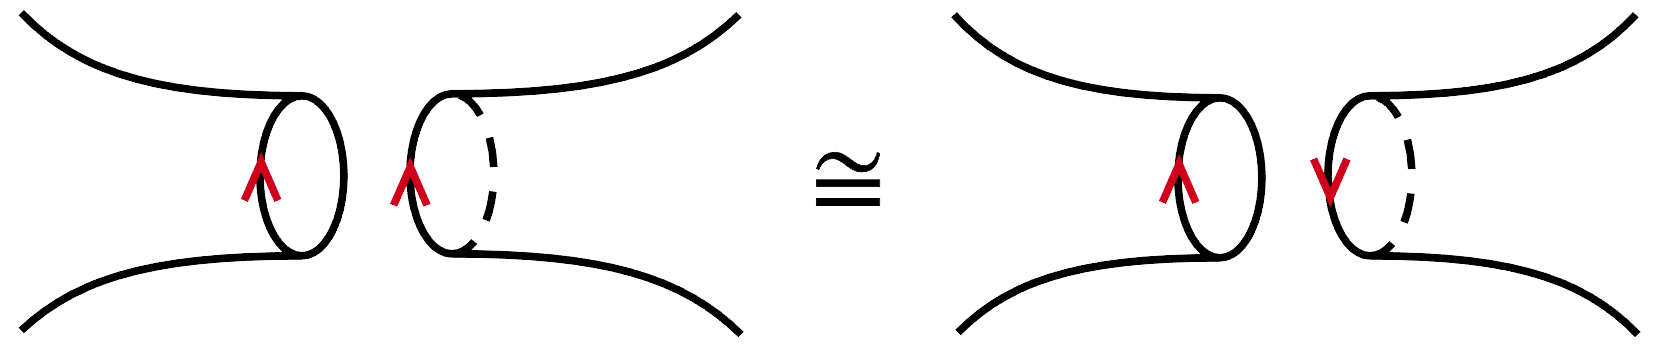
\includegraphics[width=0.8\textwidth]{fig/9.8.png}
    \captionof{figure}{粘合方式不影响连通和}
\end{figure}
\begin{figure}[h]
    \centering
    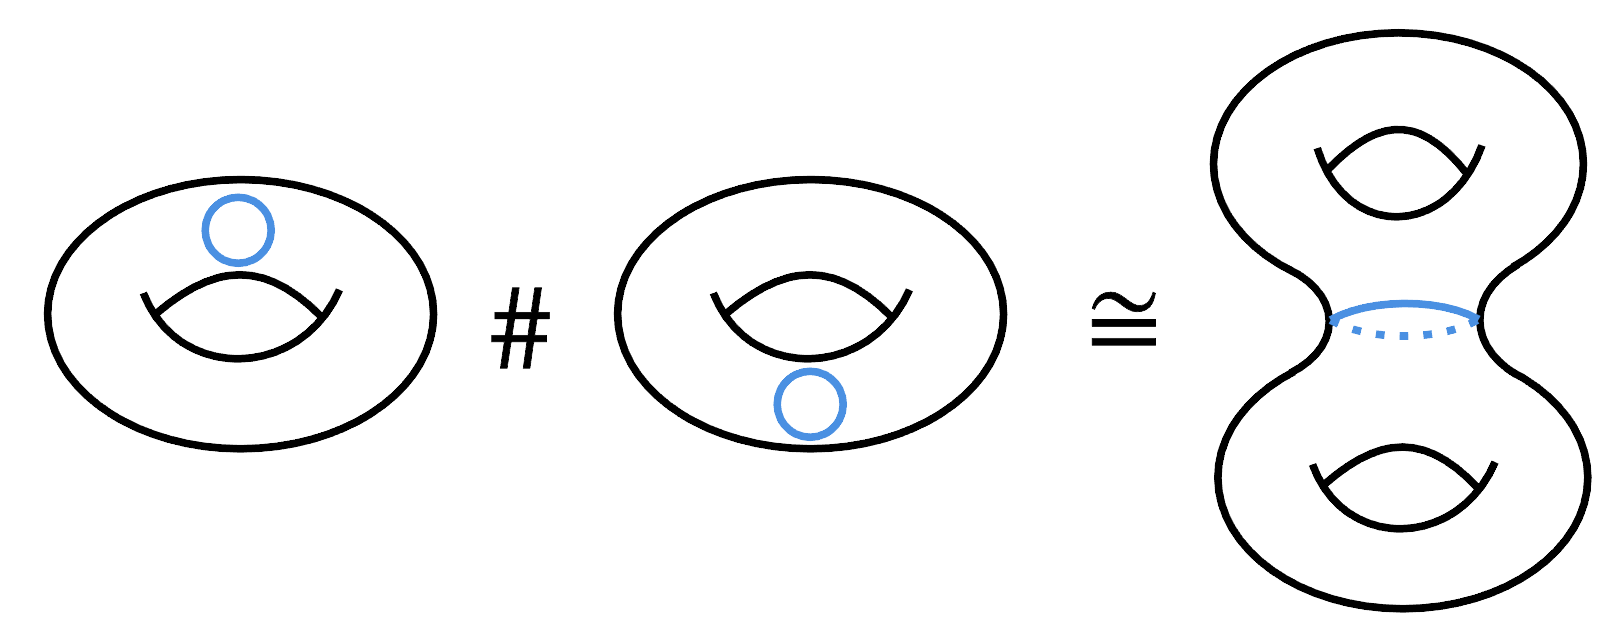
\includegraphics[width=0.8\textwidth]{fig/9.7.png}
    \captionof{figure}{移除开圆盘的位置不影响连通和}
\end{figure}


\begin{instance}
    设 $S$ 为曲面，则 $S \# S^2 \cong S$.\par
    \begin{center}
        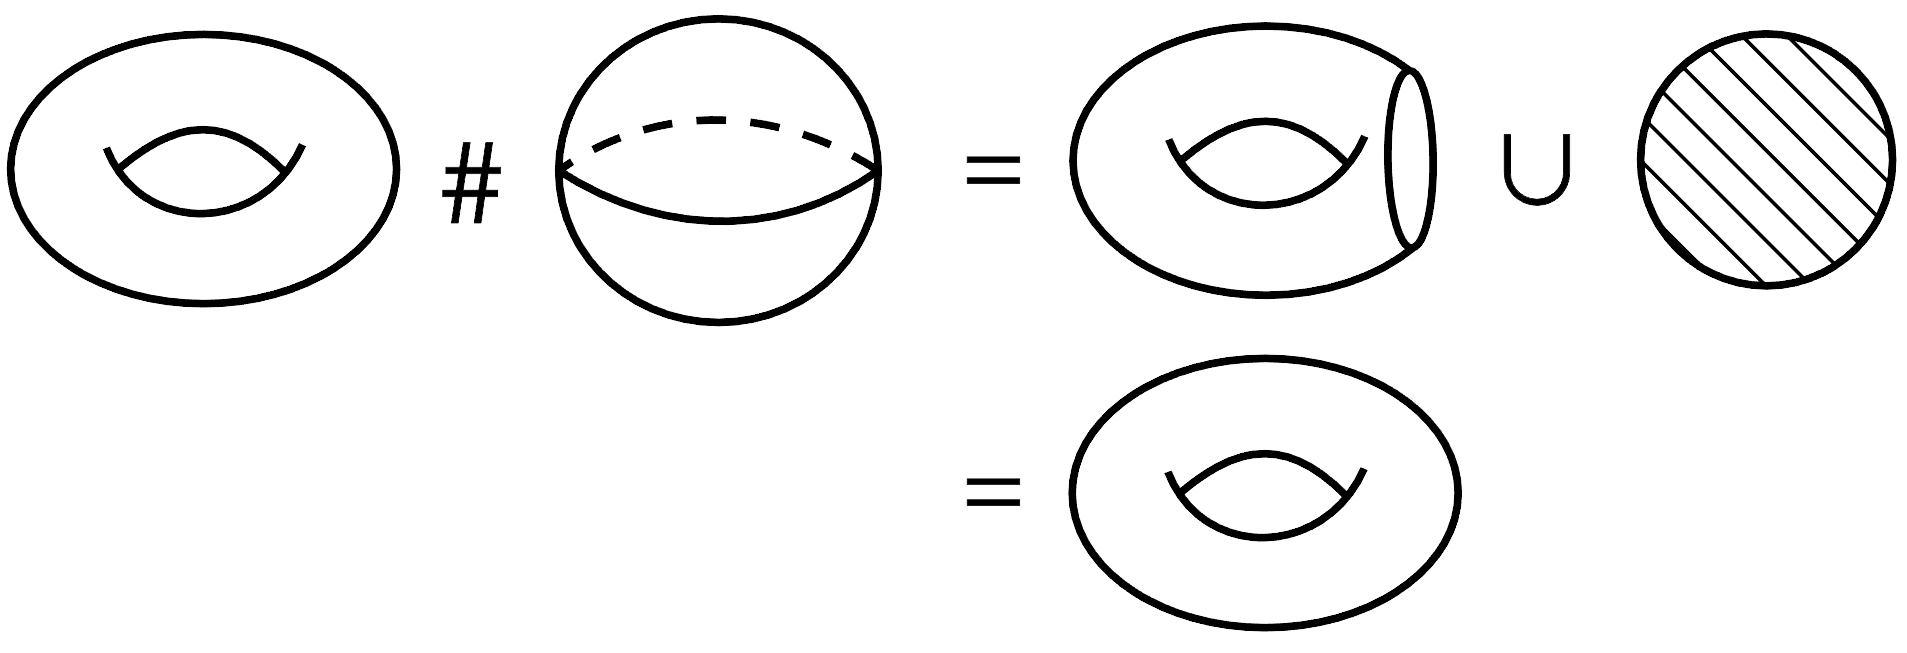
\includegraphics[width=0.8\textwidth]{fig/9.9.png}
    \captionof{figure}{}
    \end{center}
    这是因为球面挖去一个圆盘后变成了一个圆盘，因此又补上了原曲面中移除的圆盘.
\end{instance}

\begin{instance}
    环面 \# 环面 = 双环面.
    $T^2 \# T^2 \# \dots \# T^2$: $nT^2$, $n \ge 1$，可定向.
    $n$ 称为 $nT^2$ 的\bluebf{亏格}.
    \begin{center}
        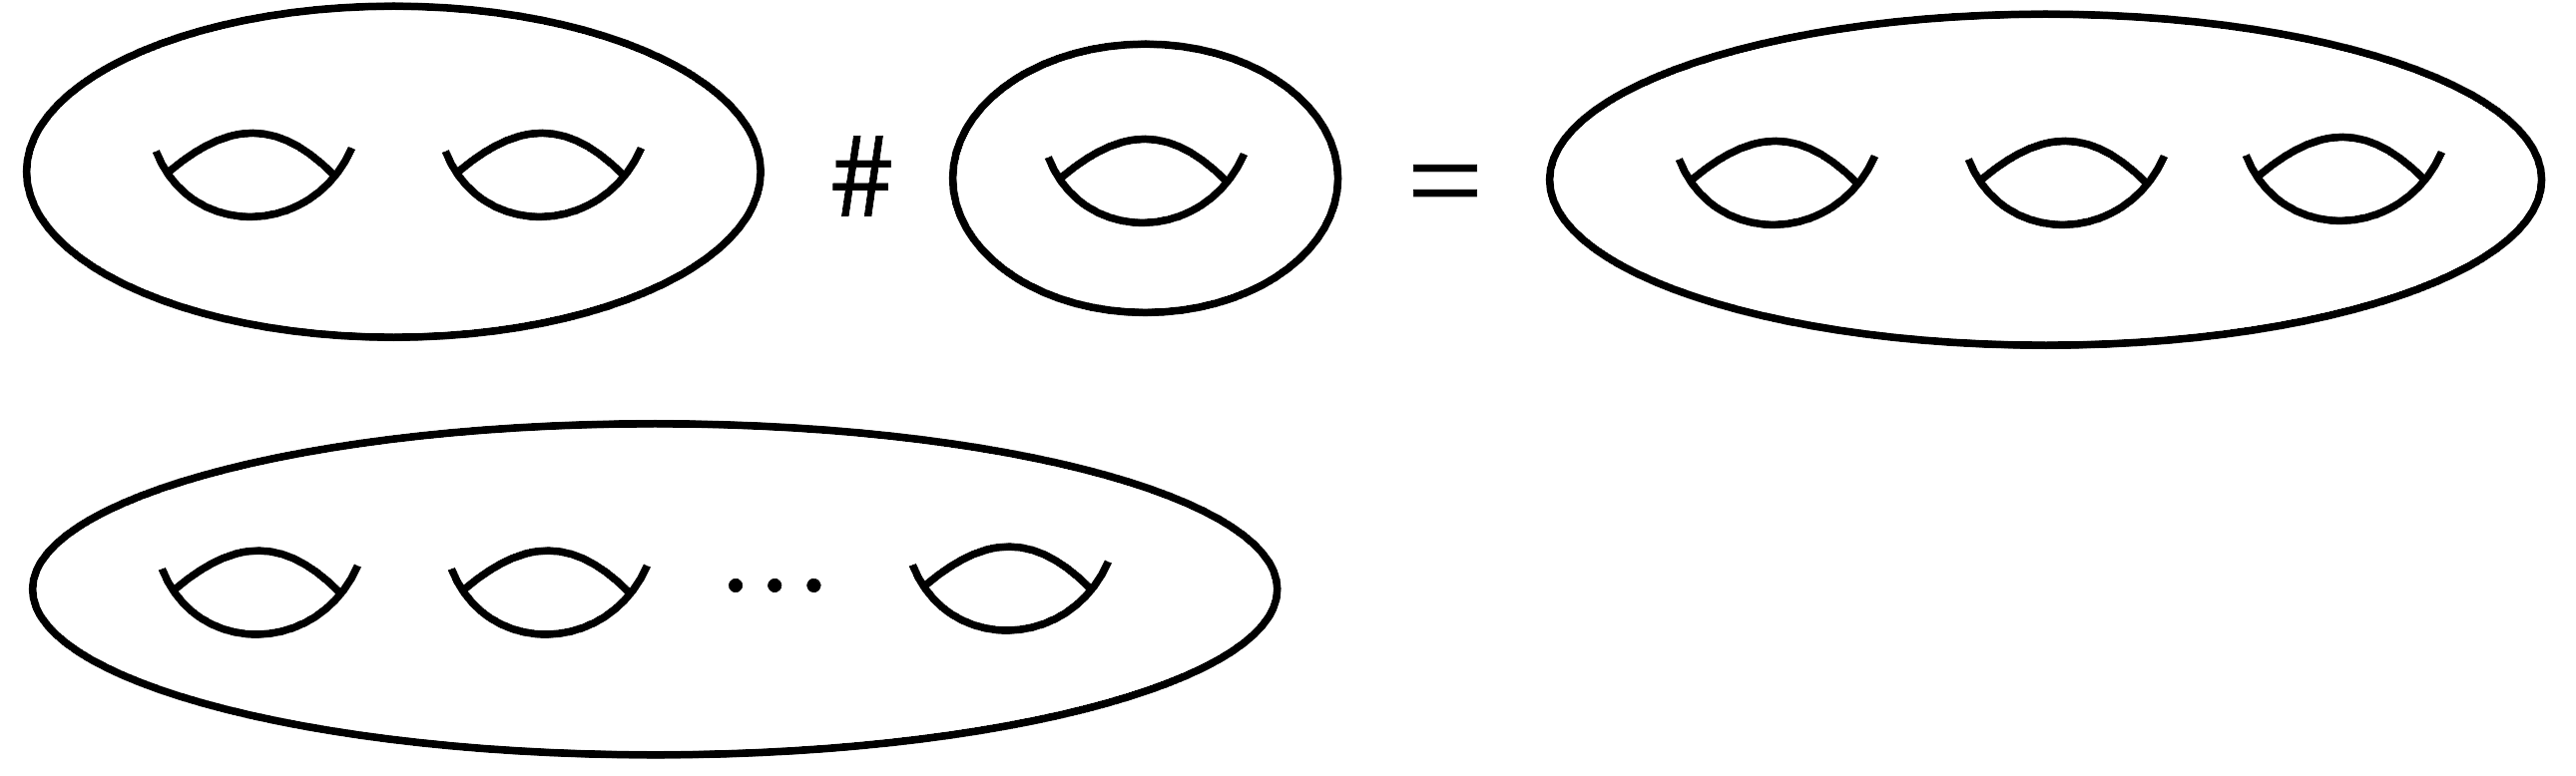
\includegraphics[width=0.8\textwidth]{fig/9.10.png}
    \captionof{figure}{}
    \end{center}
\end{instance}

\begin{instance}
    $\mathbb{R}P^2 \# \mathbb{R}P^2 \cong$ 克莱因瓶.
    \begin{center}
        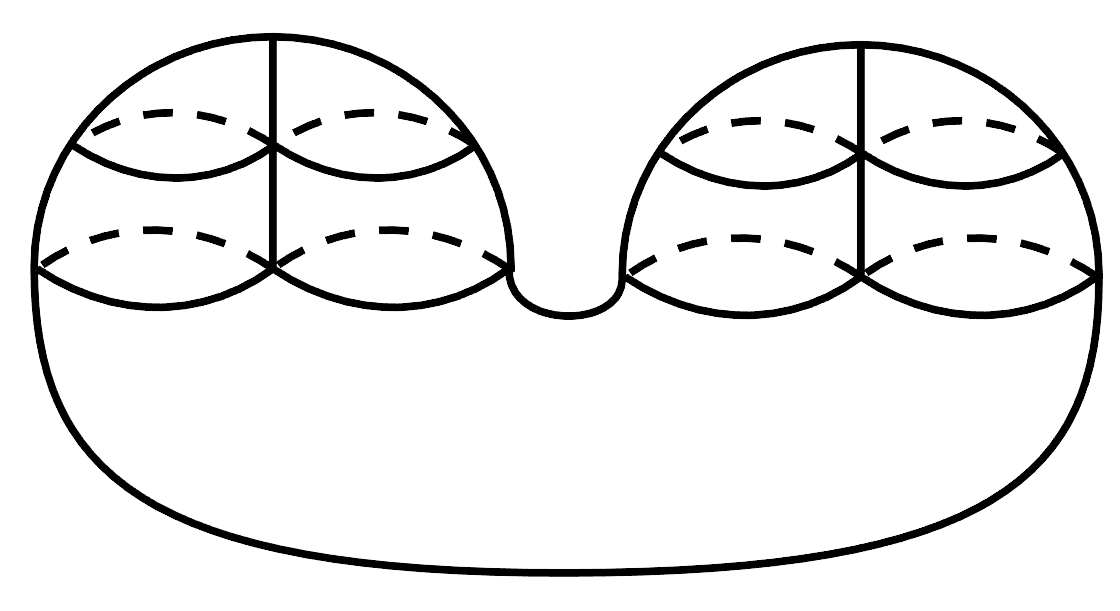
\includegraphics[width=0.3\textwidth]{fig/9.11.png}
    \captionof{figure}{}
    \end{center}
    \[ \mathbb{R}\mb{P}^2 - \mathring{D_1^2} \cup \mathbb{R}\mb{P}^2 - \mathring{D_2^2} = \text{莫比乌斯带} \cup \text{莫比乌斯带} \cong \text{克莱因瓶} \]
    $\mathbb{R}\mb{P}^2 \# \mathbb{R}\mb{P}^2 \# \dots \# \mathbb{R}\mb{P}^2$: $m\mb{P}^2$, $m \ge 1$，不可定向.
    $m$ 称为 $m\mb{P}^2$ 的\bluebf{交叉帽数}.
    \begin{center}
        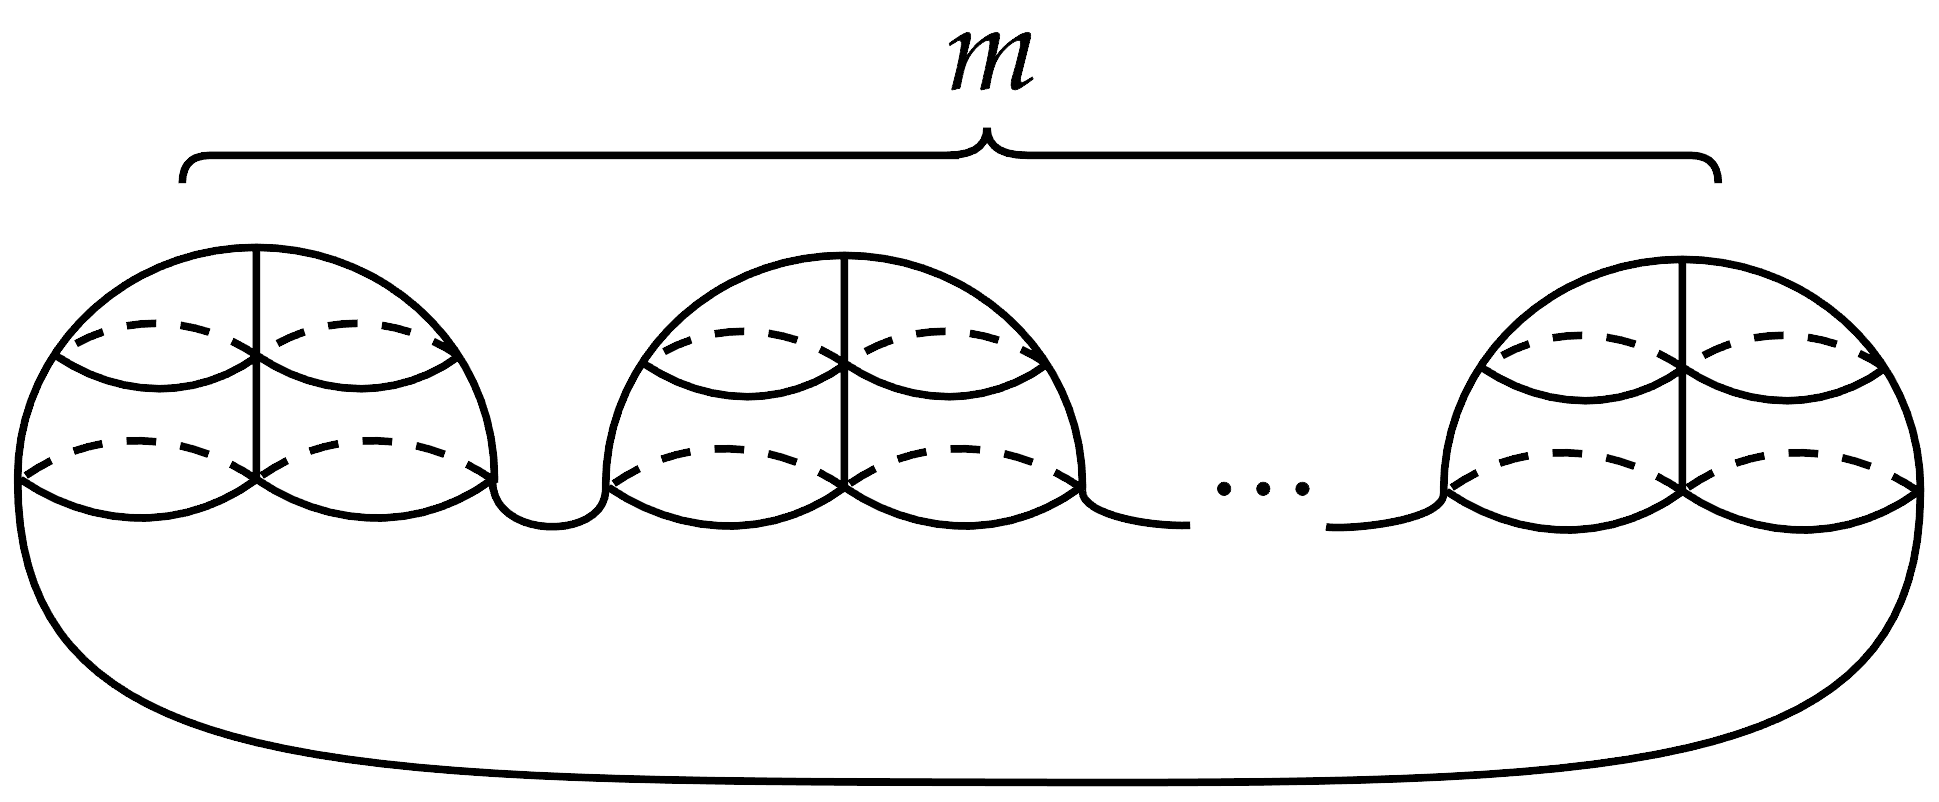
\includegraphics[width=0.7\textwidth]{fig/9.12.png}
        \captionof{figure}{}
    \end{center}
\end{instance}

\begin{instance}
    \begin{minipage}[t]{0.705\textwidth}
        $T^2 \# \mathbb{R}\mb{P}^2$ 是一个不可定向曲面.
    \end{minipage}
    \begin{minipage}[t]{0.15\textwidth}
        \vspace{-3em}
        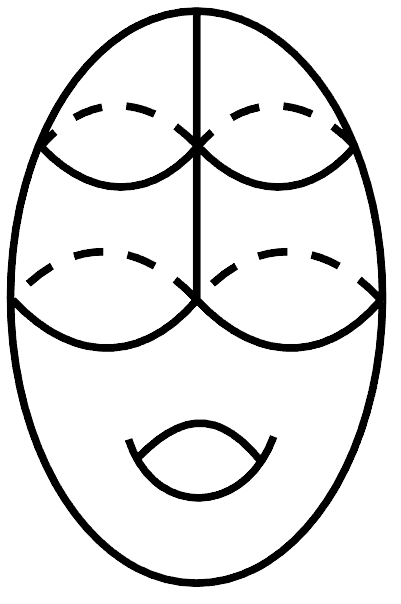
\includegraphics[width=1\textwidth]{fig/9.13.png}
        \captionof{figure}{}
    \end{minipage}
\end{instance}

\section{闭曲面的分类}

\begin{theorem}[闭曲面分类定理][thm:9.2]
    每个闭曲面同胚于 $S^2$，$nT^2$，$m\mb{P}^2$ ($n, m \ge 1$) 中的恰好一个.
\end{theorem}

\begin{instance}
    $T^2\# \mb{R}\mb{P}^2\cong 3\mb{P}^2$
\end{instance}

\begin{definition}[曲面上的三角形][def:9.5]
    设$S$是一个曲面，$S$中的一个\colorbf{三角形}是指$S$ 的一个子空间 $T$ 以及一个同胚 $h: \Delta \to T$，其中 $\Delta \subset \mathbb{E}^2$ 是一个闭三角形区域，满足
    若 $v$ 是 $\Delta$ 的顶点，则 $h(v)$ 是 $T$ 的顶点.
    若 $e$ 是 $\Delta$ 的边，则 $h(e)$ 是 $T$ 的边.
\end{definition}

\begin{definition}[三角剖分][def:9.6]
\end{definition}

\begin{instance}
    $T^2$ 的三角剖分.\par
    \begin{minipage}[t]{0.45\textwidth}
        \vspace{0em}
        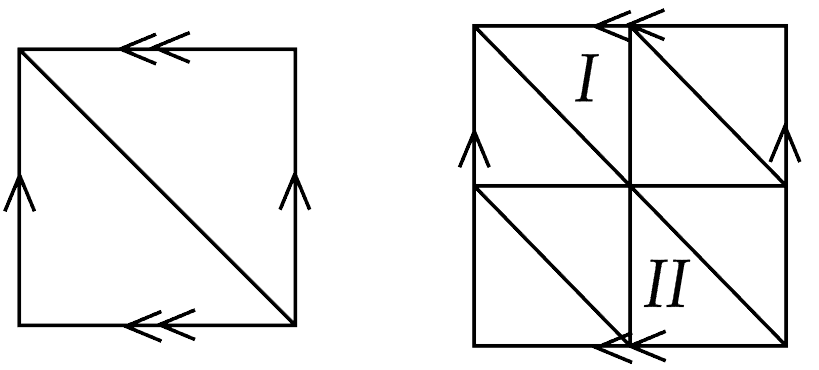
\includegraphics[width=1\textwidth]{fig/9.14.png}
        \captionof{figure}{两个错误的$T^2$的三角剖分}
    \end{minipage}
    \begin{minipage}[t]{0.45\textwidth}
        这两个均不是$T^2$的三角剖分.\par
        对于第一个图，这两个三角形相交于三条边.\par
        对于第二个图，I，II两个三角形交于两个点
    \end{minipage}
    \begin{minipage}[t]{0.45\textwidth}
    \begin{center}
        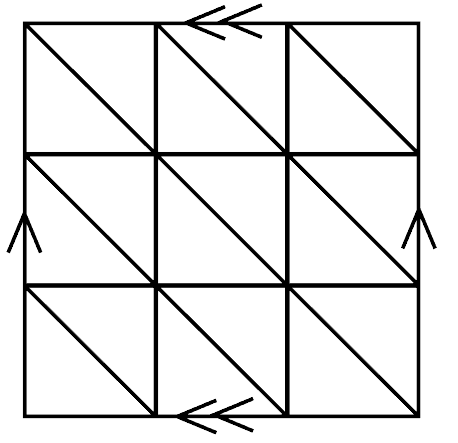
\includegraphics[width=0.5\textwidth]{fig/9.15.png}
        \captionof{figure}{$T^2$的三角剖分}
    \end{center}
    \end{minipage}
    \begin{minipage}[t]{0.45\textwidth}
    \begin{center}
        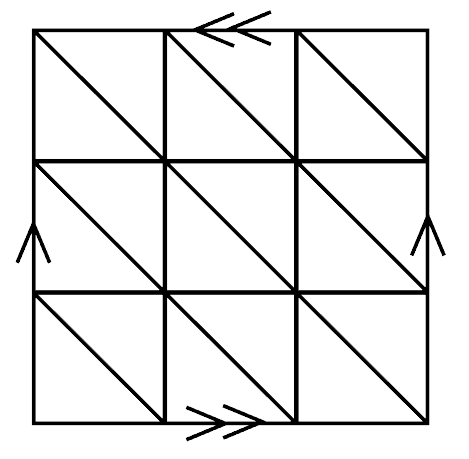
\includegraphics[width=0.5\textwidth]{fig/9.16.png}
        \captionof{figure}{克莱因瓶的三角剖分}
    \end{center}
    \end{minipage}    
\end{instance}


\begin{instance}
    $\mb{R}\mb{P}^2$ 和 $S^2$ 的三角剖分.
    \begin{center}
        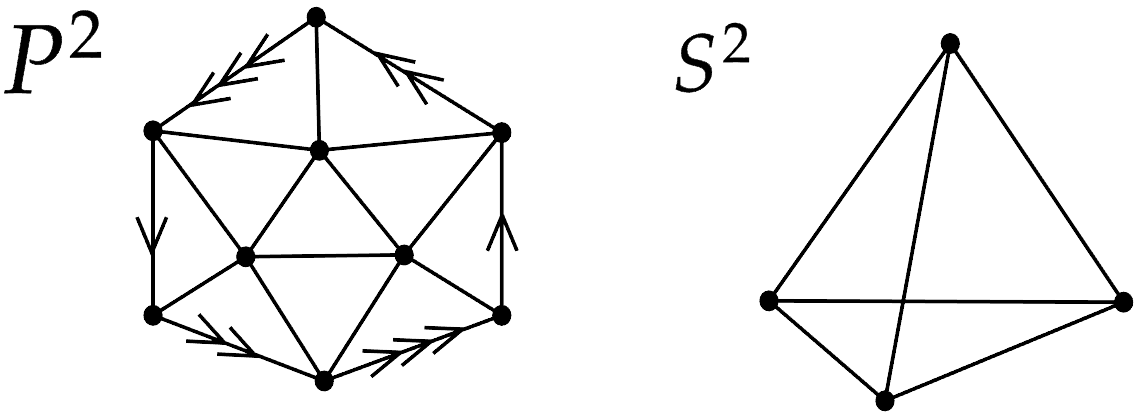
\includegraphics[width=0.6\textwidth]{fig/9.17.png}
        \captionof{figure}{}
    \end{center}
\end{instance}

\begin{theorem}[Rado, 1925][thm:9.3]
    每个闭曲面都有一个三角剖分.
\end{theorem}

\section{欧拉示性数}

\begin{definition}[欧拉示性数][def:9.7]
\index{o@欧拉示性数}
    $S$ 是一个曲面，$T$ 是 $S$ 的一个三角剖分，则$S$ 的\colorbf{欧拉示性数}定义为
    \[ \chi(S) = V - E + F \]
    其中 $V$ 是顶点数，$E$ 是边数，$F$ 是面数(三角形个数).
    $\chi(S)$ 不依赖于 $T$ 的选取.
\end{definition}

\begin{instance}
    $\chi(T^2) = 9 - 27 + 18 = 0$\hspace{4em}
    $\chi(K) = 9 - 27 + 18 = 0$\par
    \hspace{2.5em}$\chi(\mathbb{R}\mb{P}^2) = 6 - 15 + 10 = 1$\hspace{4em}
    $\chi(S^2) = 4 - 6 + 4 = 2$
\end{instance}

\begin{lemma}[][lem:9.1]
    \[ \chi(S_1 \# S_2) = \chi(S_1) + \chi(S_2) - 2 \]
\end{lemma}
\begin{proof}
    利用三角剖分证明.
    设 $\chi(S_1) = V_1 - E_1 + F_1$，$\chi(S_2) = V_2 - E_2 + F_2$.
    在进行连通和操作时，我们移除两个面（每个曲面一个），则
    {\setjot[-6]\begin{align*}
    \chi(S_1 \# S_2)&= (V_1 + V_2 - 3) - (E_1 + E_2 - 3) + (F_1 + F_2 - 2)\\
    &= (V_1 - E_1 + F_1) + (V_2 - E_2 + F_2) - 2\\ 
    &= \chi(S_1) + \chi(S_2) - 2
    \end{align*}}
\end{proof}

\begin{instance}
    $\chi(nT^2) = 2 - 2n, \quad \chi(m\mb{P}^2) = 2 - m$
\end{instance}

\section{曲面的多边形表示}

\begin{definition}[多边形表示][def:9.8]
\end{definition}

\begin{proposition}[][prop:9.1]
    任意闭曲面都有一个多边形表示.
\end{proposition}

\begin{remark}
    一个闭曲面可以有多个多边形表示.
\end{remark}

\begin{instance}
    环面$T^2$的一个多边形表示，可以用$aba^{-1}b^{-1}$表示 \par
    \begin{minipage}{0.22\textwidth}
        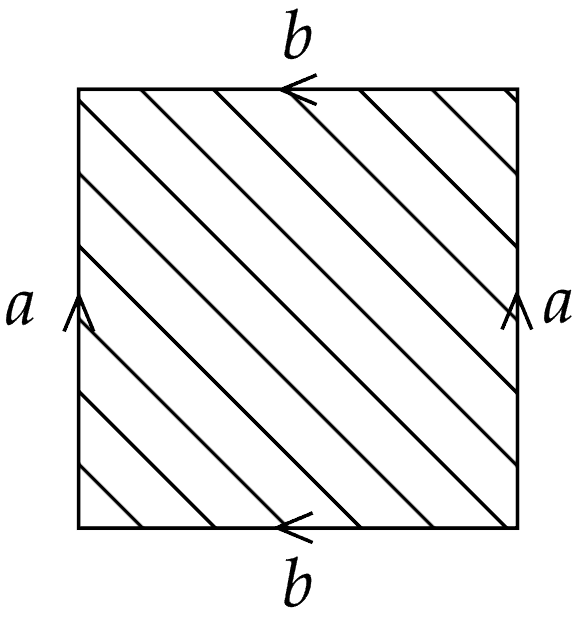
\includegraphics[width=0.98\textwidth]{fig/9.18.png}
        \captionof{figure}{}
    \end{minipage}
    \begin{minipage}{0.72\textwidth}
        \begin{center}
        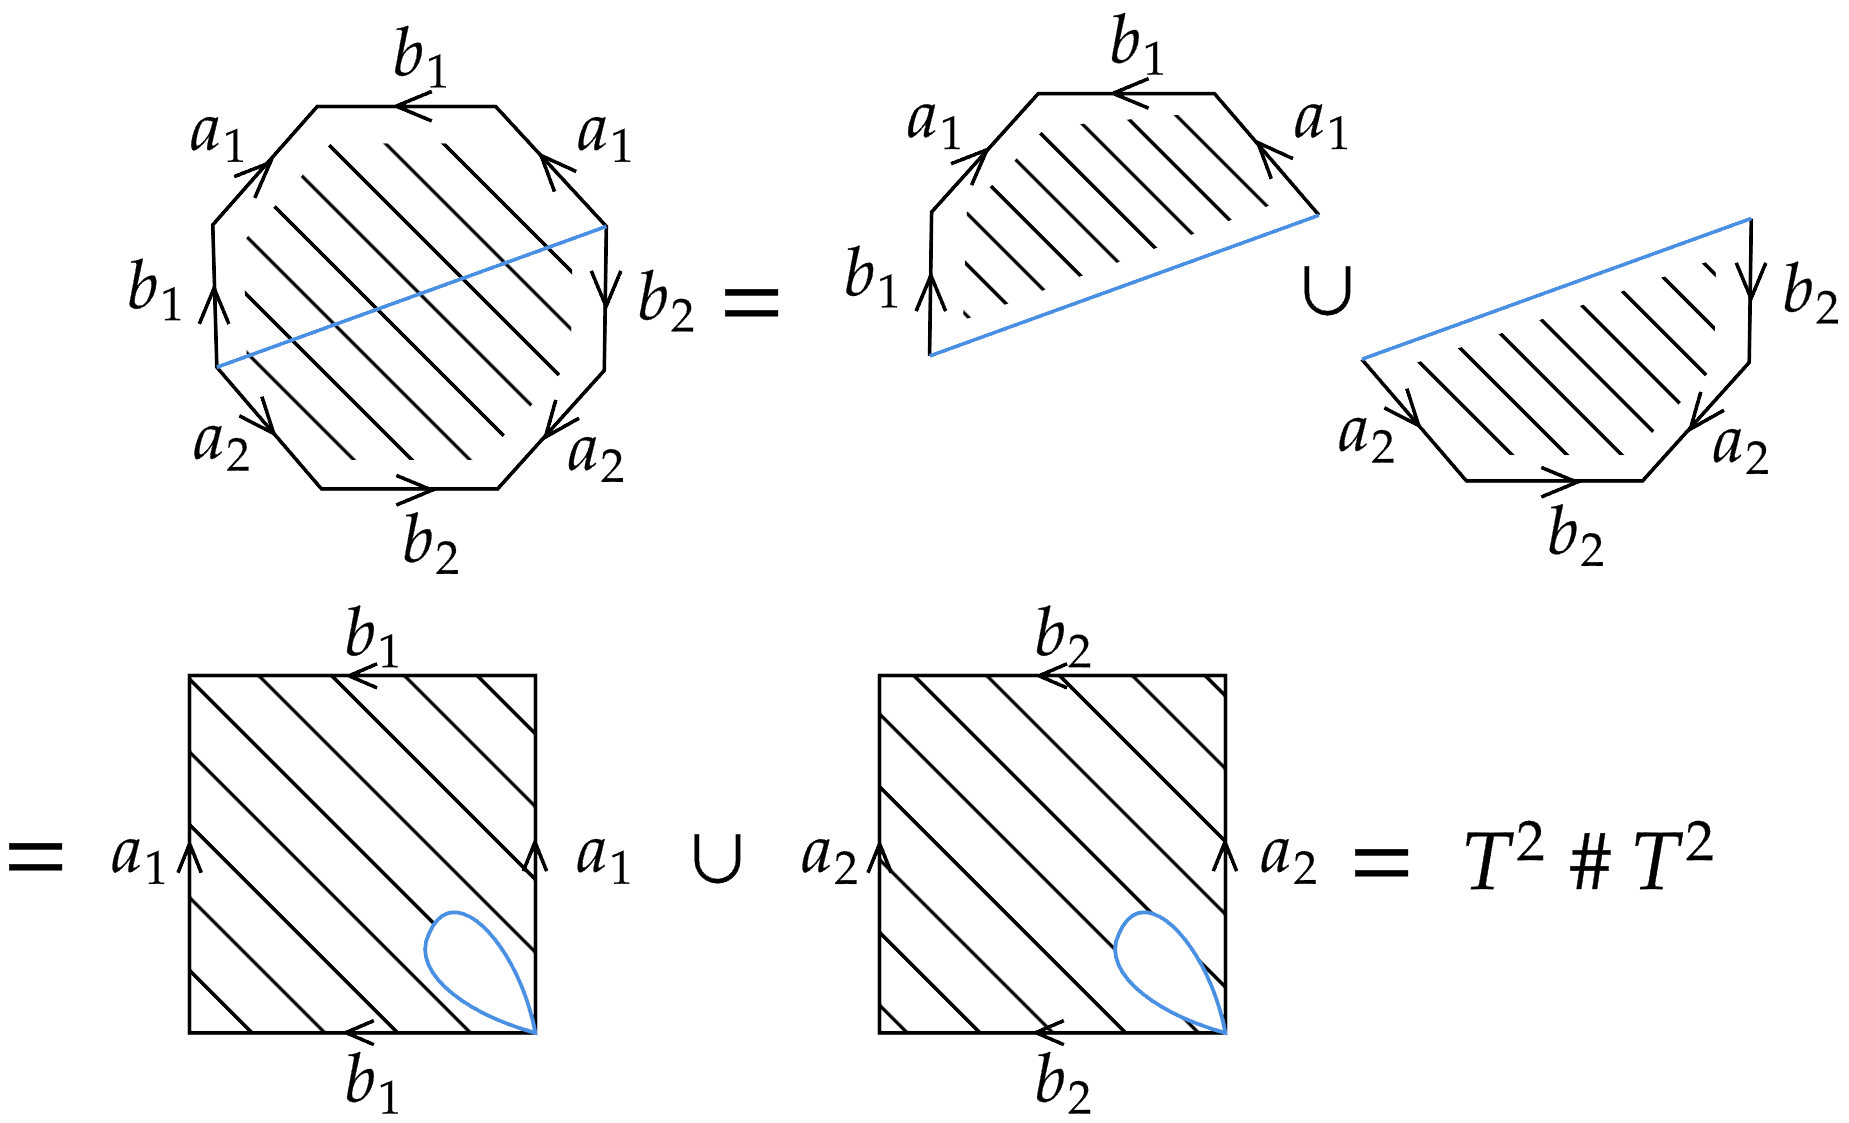
\includegraphics[width=0.98\textwidth]{fig/9.19.png}
        \captionof{figure}{}
    \end{center}
    \end{minipage}\par
    $T^2\# T^2$的一个多边形表示，可以用$a_1b_1a_1^{-1}b_1^{-1}a_2b_2a_2^{-1}b_2^{-1}$表示
\end{instance}



\begin{instance}
    类似地，有$3T^2$: $a_1 b_1 a_1^{-1} b_1^{-1} a_2 b_2 a_2^{-1} b_2^{-1} a_3 b_3 a_3^{-1} b_3^{-1}$.\par
    $nT^2=a_1b_1a_1^{-1}b_1^{-1}\cdots a_nb_na_n^{-1}b_n^{-1}$
    \begin{center}
        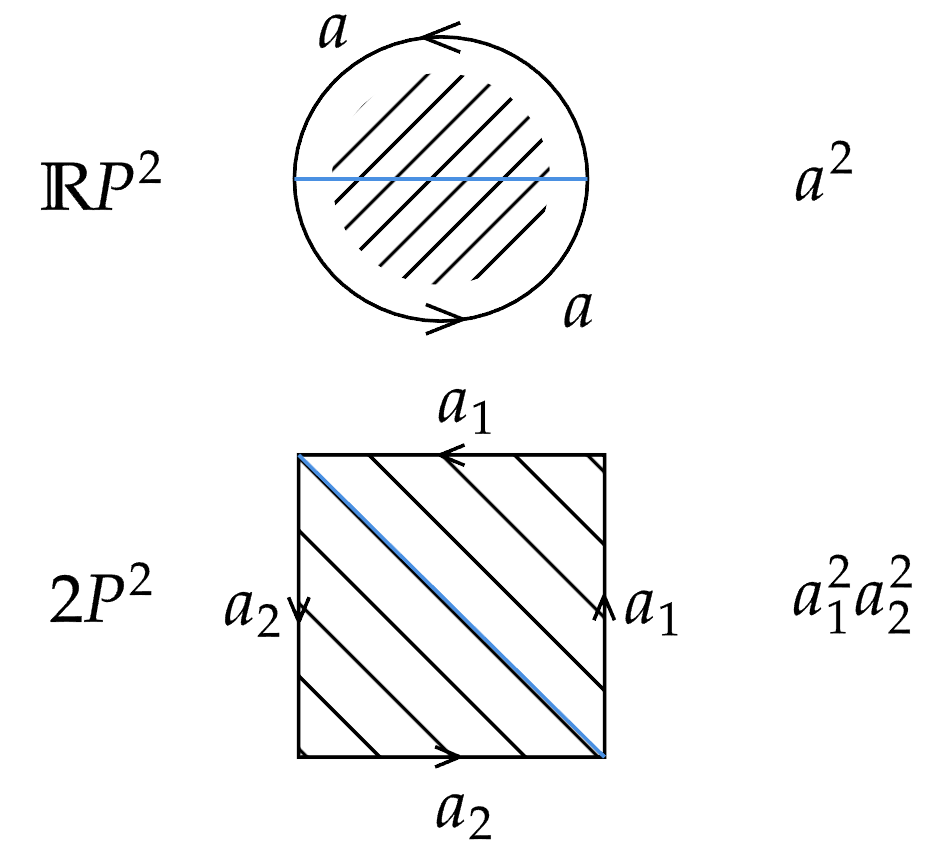
\includegraphics[width=0.45\textwidth]{fig/9.20.png}
    \end{center}
    \begin{center}
        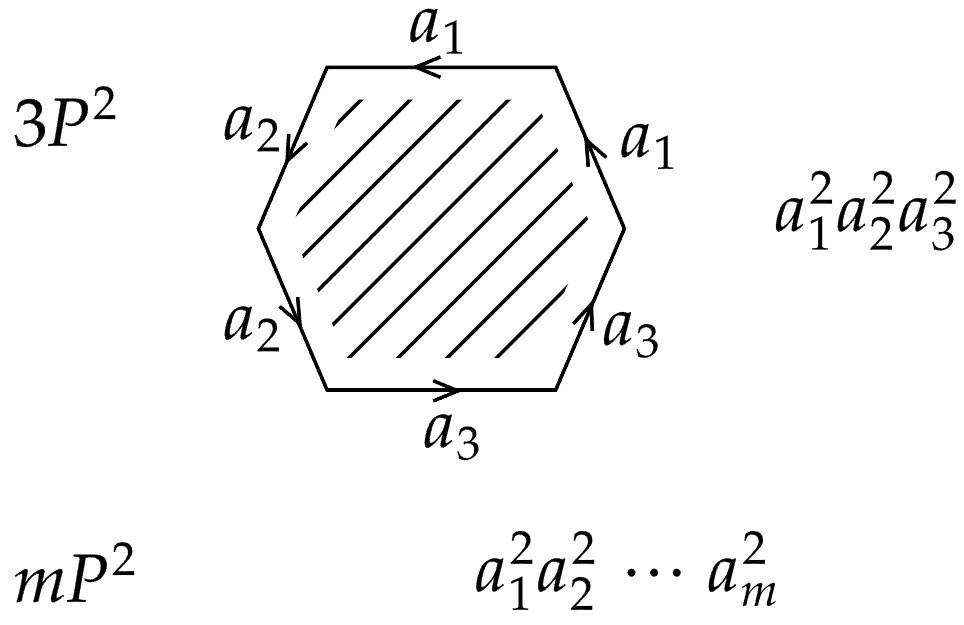
\includegraphics[width=0.45\textwidth]{fig/9.20-2.png}
        \captionof{figure}{}
    \end{center}
\end{instance}


\subsection{标准多边形表示}



\begin{theorem}[][thm:9.4]
    任意多边形表示都可以变换为标准形式.\par
    \begin{itemize}
    \item $nT^2$: $a_1 b_1 a_1^{-1} b_1^{-1} \dots a_n b_n a_n^{-1} b_n^{-1}$
    \item $m\mb{P}^2$: $a_1^2 a_2^2 \dots a_m^2$
\end{itemize}
\end{theorem}

\begin{instance}
    非标准形式 $\leadsto$ 标准形式.
    \begin{center}
        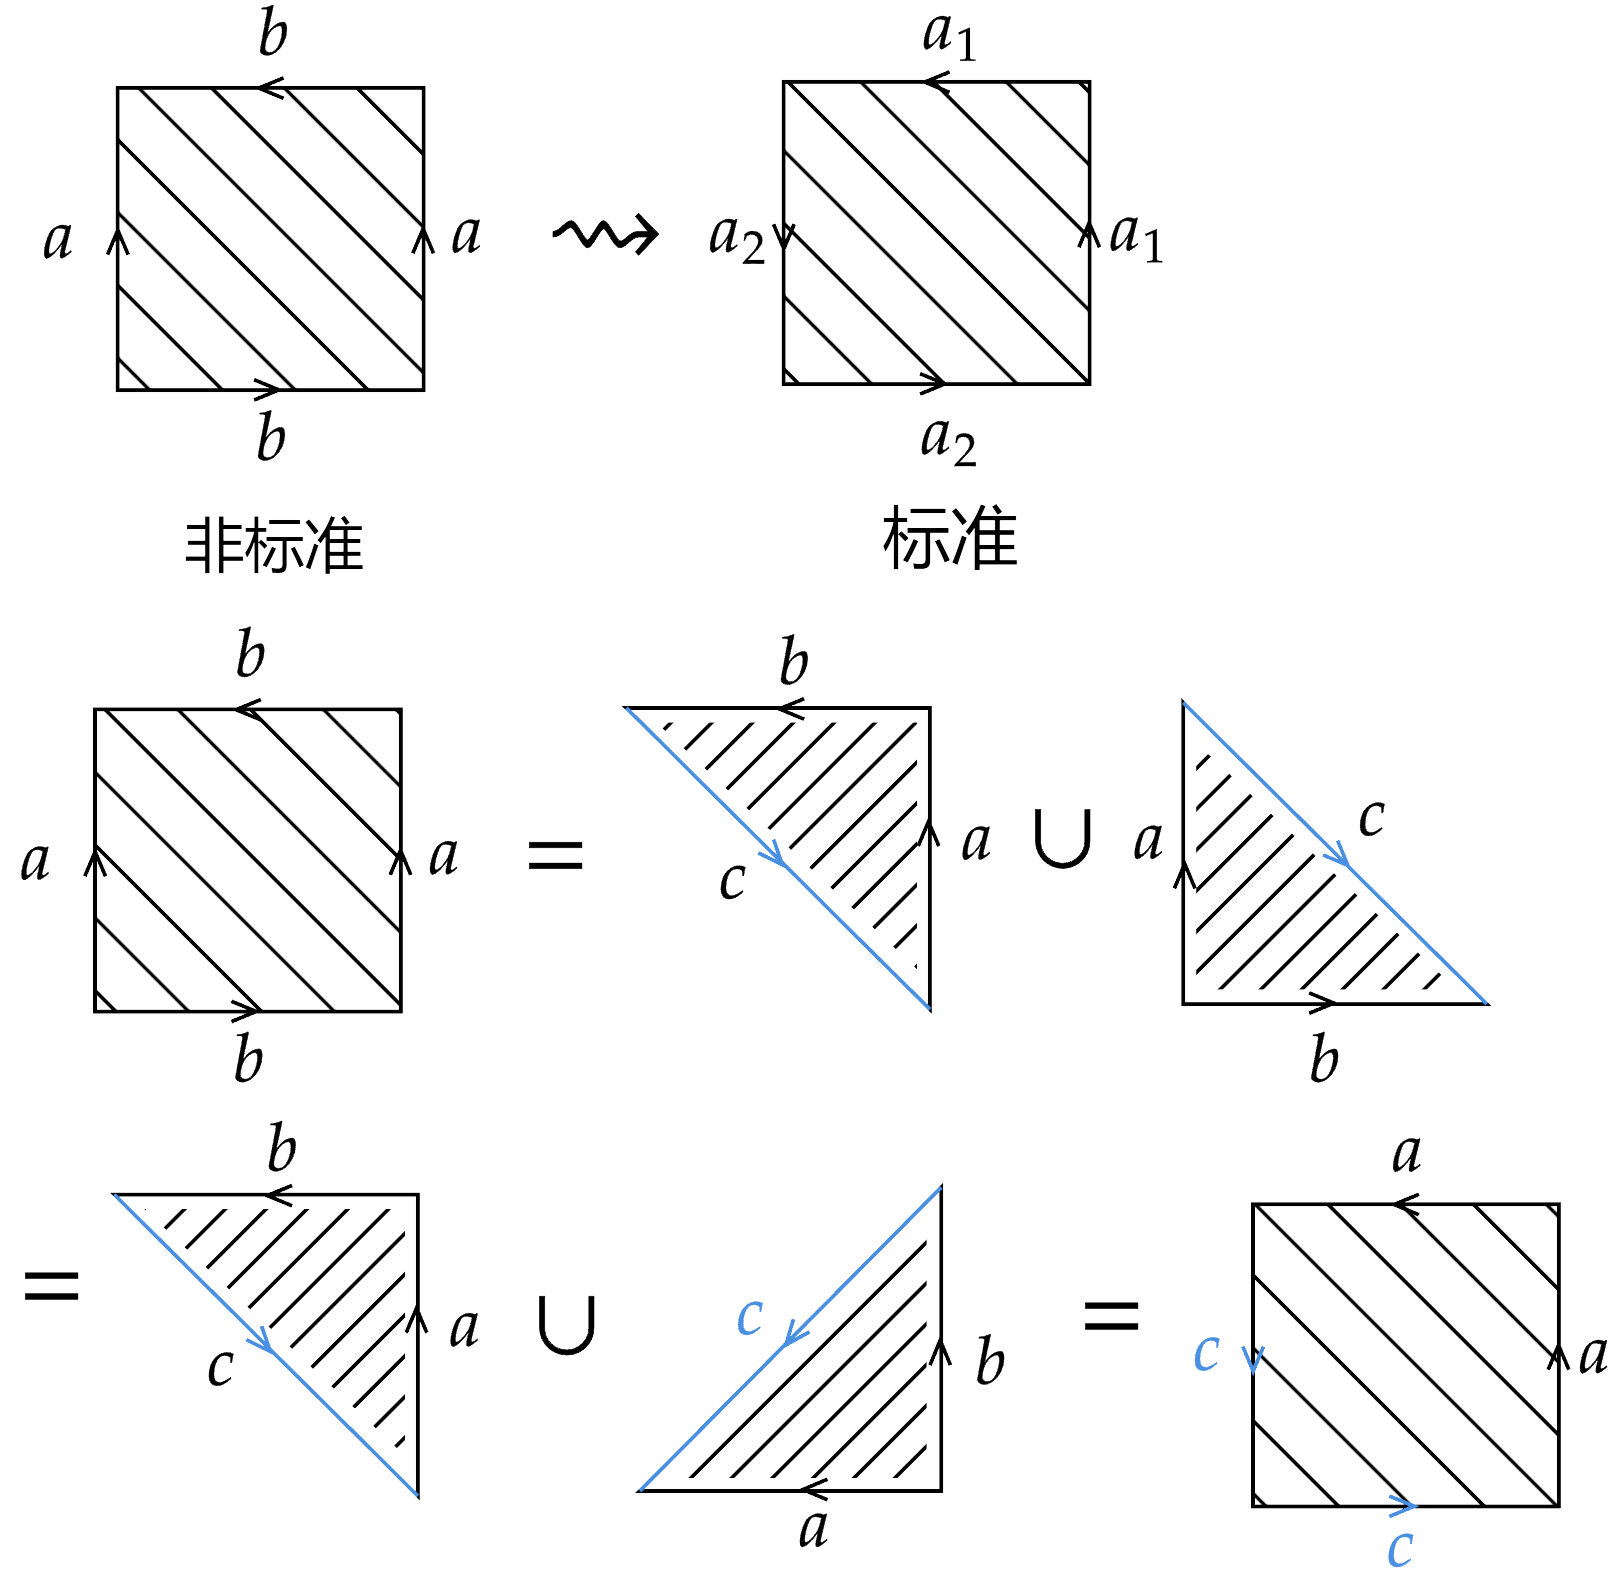
\includegraphics[width=0.7\textwidth]{fig/9.21.png}
        \captionof{figure}{}
    \end{center}
\end{instance}


\subsection{曲面多边形表示的标准化}

\textbf{顶点类}：粘合在一起的顶点.

\textbf{反向对}：$\vcenter{\hbox{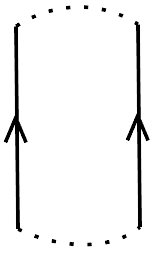
\includegraphics[width=0.1\textwidth]{fig/9.a-1.png}}}$
\textbf{同向对}：$\vcenter{\hbox{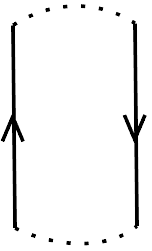
\includegraphics[width=0.1\textwidth]{fig/9.a-2.png}}}$

\textbf{手术 A}：
\begin{center}
    \vspace{-1.5 em}
    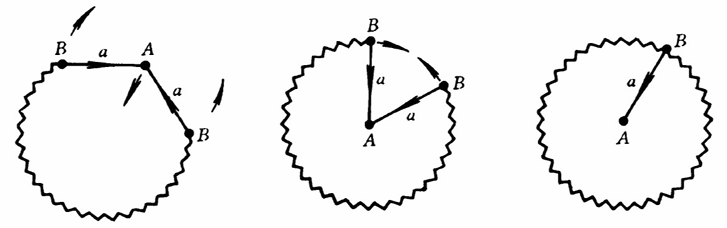
\includegraphics[width=0.7\textwidth]{fig/9.22.png}
    \captionof{figure}{}
\end{center}

\textbf{手术 B}：
\begin{center}
    \vspace{-1.5 em}
    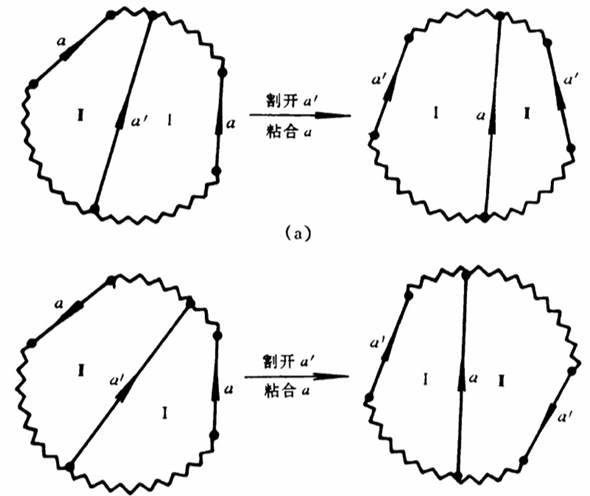
\includegraphics[width=0.7\textwidth]{fig/9.23.png}
    \captionof{figure}{}
\end{center}

“多边形有无同向对”这一性质不会被手术 A，B 改变，但同向对的数量可能改变.

\subsubsection{1. 减少多边形的边数（即减少顶点类数）}

设有 $l$ 条边，$k$ 个顶点类.

设 $(\tau, \varphi)$ 的顶点类数 $k > 1$.取其中一类，记作 $P$.

\textbf{1.1}\; $P$ 中只有 1 个顶点，则只有$\vcenter{\hbox{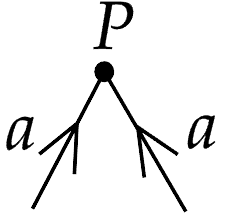
\includegraphics[width=0.1\textwidth]{fig/9.a.png}}}$或$\vcenter{\hbox{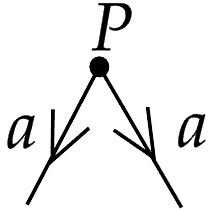
\includegraphics[width=0.1\textwidth]{fig/9.b.png}}}$.
作手术 A，消灭 $P$.


\textbf{1.2}\; $P$ 中不只有一个顶点.
\begin{center}
    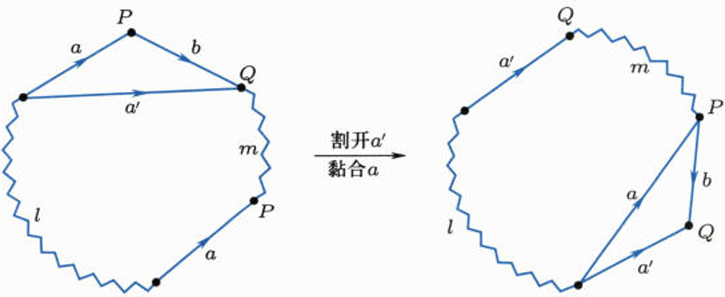
\includegraphics[width=0.8\textwidth]{fig/9.24.png}
    \captionof{figure}{}
\end{center}\par
顶点类数 $>1$，存在一个 $P$ 类顶点与 $Q$ 类顶点相邻，$a \neq b$.作手术 B，减少一个 $P$ 类顶点，增加一个 $Q$ 类顶点.\par
重复多次，把 $P$ 类顶点减少至 1 个.回到 1.1，作手术 A，消灭 $P$ 类顶点.\par
重复多次，只剩下的一个顶点类.

结果：$l - 2(k-1)$ 条边，1 个顶点类.

\subsubsection{2. 改变粘合方式}

此时 $(\tau', \varphi')$ 只有一个顶点类.

\begin{lemma}[][lem:9.2]
    $(\tau, \varphi)$ 中的反向对不相邻，且至少与另一边对相间排列.
\end{lemma}
\begin{proof}
    如果反向对相邻$\vcenter{\hbox{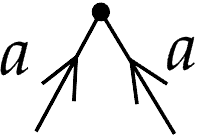
\includegraphics[width=0.1\textwidth]{fig/9.c.png}}}$，则顶点类数 $>1$，矛盾.\par
    \begin{minipage}[t]{0.25\textwidth}
        \vspace{-1em}
        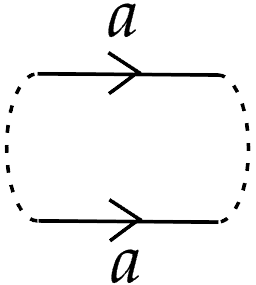
\includegraphics[width=0.8\textwidth]{fig/9.d.png}
    \end{minipage}
    \begin{minipage}[t]{0.65\textwidth}
        \vspace{3 em}
         如果左侧的边不与右侧的边粘合，则左侧顶点不与右侧顶点等价，则顶点类数 $>1$，矛盾.
    \end{minipage}\par
\end{proof}

\textbf{2.1} 无同向对.
\begin{center}
    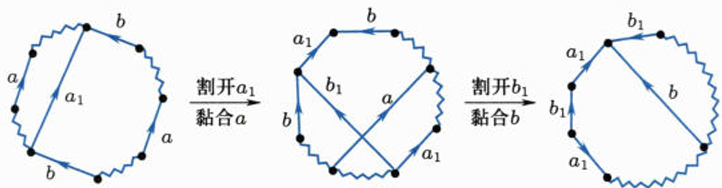
\includegraphics[width=0.9\textwidth]{fig/9.25.png}
    \captionof{figure}{对$a,b$分别作手术B}
\end{center}\par
$a$ 是反向对，由引理，存在另一反向对 $b$ 与 $a$ 相间排列.利用手术 B，消去 $a$ 和 $b$，增加相间排列并且相邻的反向对 $a_1$ 和 $b_1$.
重复多次可得 $a_1 b_1 a_1^{-1} b_1^{-1} \dots a_n b_n a_n^{-1} b_n^{-1}$.

\textbf{2.2} 有同向对.
\begin{center}
    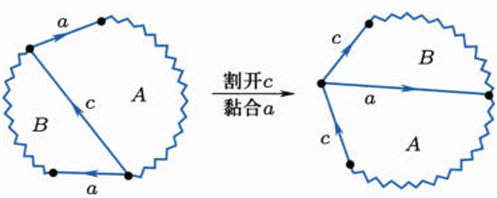
\includegraphics[width=0.8\textwidth]{fig/9.26.png}
    \captionof{figure}{用$(c,a)$作手术B}
\end{center}\par
做手术 B，产生一个相邻的同向对.
重复多次，使得无不相邻的同向对.

\textbf{2.2.1} 若没有反向对，则得到标准型
\[ a_1 a_1 \dots a_m a_m \]

\textbf{2.2.2} 若有反向对.设 $a$ 是反向对.
由引理，边对 $b$ 与 $a$ 相间排列.因同向对都相邻，$b$ 是反向对.
\begin{center}
    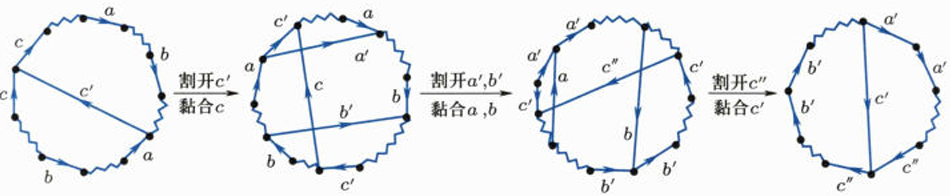
\includegraphics[width=0.95\textwidth]{fig/9.27.png}
\end{center}\par
利用手术 B，消灭 $a, b$，增加同向对 $a', b'$.
同时，把同向对变为相邻.重复多次，得到标准型 $a_1 a_1 \dots a_m a_m$.

\subsection{总结}

1. 判断有无同向对.

2. 有：$\frac{l - 2(k-1)}{2} P^2$；无：$\frac{l - 2(k-1)}{4} T^2$.
其中 $k$ 为顶点类数，$l$ 为边数.

\begin{instance}
    \[ nT^2 \# mP^2 \cong (2n+m)P^2 \]
    \[ a_1 b_1 a_1^{-1} b_1^{-1} \dots a_n b_n a_n^{-1} b_n^{-1} c_1^2 \dots c_m^2 \]
    1 个顶点类，$4n+2m$ 条边.有同向对.
    所以为 $(2n+m)P^2$.
\end{instance}

\section{流形}

\begin{definition}[n维流形][def:9.9]
    \[ \mathbb{E}^n_+ = \{ (x_1, \dots, x_n) \in \mathbb{E}^n \mid x_n \ge 0 \} \]
\end{definition}

\begin{proposition}[][prop:9.2]
    流形是可度量化的.
\end{proposition}
\begin{proof}
    利用 Urysohn 度量化定理.
    正则 + 第二可数 $\implies$ 可度量化.
\end{proof}



